\documentclass[12pt,a4paper]{article}

\usepackage[utf8]{inputenc}
\usepackage[T1]{fontenc}
\usepackage[margin=1in]{geometry}
\usepackage{amsmath,amssymb,amsthm}
\usepackage{graphicx}
\usepackage{hyperref}
\usepackage{listings}
\usepackage{xcolor}
\usepackage{enumitem}
\usepackage{fancyhdr}
\usepackage{tcolorbox}
\usepackage{booktabs}
\usepackage{makecell}
\usepackage{placeins}
\usepackage{tabularx}
	\usepackage{biblatex}
\addbibresource{reference.bib} 
\usepackage{tikz}
\usetikzlibrary{shapes,arrows,positioning,fit,backgrounds,calc}
\usepackage{rotating}

\usepackage{tikz}
\usepackage{caption}
\usepackage{listing}
\usetikzlibrary{shapes, arrows.meta, positioning, fit}


\lstset{
    basicstyle=\ttfamily\small,
    keywordstyle=\color{blue},
    commentstyle=\color{gray},
    stringstyle=\color{red},
    numbers=left,
    numberstyle=\tiny\color{gray},
    stepnumber=1,
    numbersep=5pt,
    backgroundcolor=\color{white},
    showspaces=false,
    showstringspaces=false,
    showtabs=false,
    frame=single,
    tabsize=2,
    captionpos=b,
    breaklines=true,
    breakatwhitespace=false
}

\newtcolorbox{keypoint}{
    colback=blue!5!white,
    colframe=blue!75!black,
    title=Key Point
}

\newtcolorbox{example}{
    colback=green!5!white,
    colframe=green!75!black,
    title=Example
}

\newtcolorbox{exercise}{
    colback=orange!5!white,
    colframe=orange!75!black,
    title=Exercise
}

\newtcolorbox{warning}{
    colback=red!5!white,
    colframe=red!75!black,
    title=Common Pitfall
}

\theoremstyle{definition}
\newtheorem{definition}{Definition}[section]
\newtheorem{theorem}{Theorem}[section]
\newtheorem{lemma}[theorem]{Lemma}
\newtheorem{proposition}[theorem]{Proposition}

\pagestyle{fancy}
\fancyhf{}
\lhead{\coursename}
\rhead{Topic: \topicname}
\cfoot{\thepage}

\newcommand{\coursename}{Foundations of Quantitative Social Science Research}
\newcommand{\topicname}{Introduction}
\newcommand{\lecturenum}{Lecture 1}
\newcommand{\instructor}{Wanhong Huang}
\newcommand{\semester}{Spring 2025}

\title{\textbf{\coursename} \\ \lecturenum: \topicname}
\author{\instructor}
\date{\semester}


\begin{document}
\maketitle

\tableofcontents
\newpage


\section{Learning Objectives}

By the end of this session, students will be able to:

\begin{enumerate}
    \item \textbf{Understand the complete research lifecycle in quantitative social science}
    \begin{itemize}
        \item Identify and describe the six stages of the quantitative research lifecycle: question discovery, research design, data collection, data processing, data analysis, and dissemination
        \item Explain how these stages interconnect and iterate throughout a research project
        \item Recognize stage-specific methodological considerations and challenges
    \end{itemize}
    
    \item \textbf{Distinguish among major research schemes in quantitative social science}
    \begin{itemize}
        \item Characterize the distinctive features, advantages, and limitations of literature review and meta-analysis, experimental research, survey research, document and content analysis, and secondary data analysis
        \item Match appropriate research schemes to specific research questions and contexts
        \item Understand how different schemes instantiate the common research lifecycle with distinct emphases
    \end{itemize}
    
    \item \textbf{Recognize the landscape of data analysis methods}
    \begin{itemize}
        \item Categorize major families of analytical methods: statistics-based, information theory-based, machine learning, network analysis, and interdisciplinary-integrated approaches
        \item Identify representative techniques within each methodological tradition
        \item Appreciate the complementary roles of different analytical approaches in addressing research questions
    \end{itemize}
    
    \item \textbf{Identify key challenges in contemporary quantitative social science research}
    \begin{itemize}
        \item Articulate the problem of data and tool fragmentation across methodological traditions and software ecosystems
        \item Explain research lifecycle discontinuity and its implications for workflow efficiency and information propagation
        \item Describe structural reproducibility deficits arising from inadequate documentation infrastructure
        \item Recognize steep learning curves resulting from insufficient abstraction in current tools
        \item Understand data heterogeneity and scale challenges in modern multi-source, multimodal research
    \end{itemize}
    
    \item \textbf{Envision requirements for an integrative computational research framework}
    \begin{itemize}
        \item Understand how unified data architecture addresses heterogeneity and scale challenges
        \item Recognize the role of standardized workflow abstractions in supporting lifecycle continuity
        \item Appreciate integrated analytical methods as solutions to tool fragmentation
        \item Explain how computational reproducibility infrastructure enables verification and extension of research
        \item Identify opportunities for intelligent assistance and progressive abstraction to reduce learning barriers
    \end{itemize}
    
    \item \textbf{Develop critical awareness of research infrastructure and tools}
    \begin{itemize}
        \item Evaluate current tools and platforms in terms of their support for different research lifecycle stages
        \item Recognize trade-offs between flexibility and usability, specialization and integration
        \item Understand visualization and reporting tools appropriate for different audiences and purposes
        \item Appreciate the importance of reproducibility tools including code repositories, computational notebooks, and containerization
    \end{itemize}
\end{enumerate}


\section{Overview}

This introductory session provides a comprehensive map of the quantitative social science research landscape, establishing foundational concepts and frameworks that will guide subsequent course content. We approach quantitative social science as a systematic enterprise characterized by a common research lifecycle, diverse research schemes that instantiate this lifecycle in distinct ways, and an expanding repertoire of analytical methods and computational tools.

\subsection*{The Research Lifecycle Framework}

We begin by establishing the six-stage research lifecycle as our organizing framework: (1) question discovery, where research problems emerge from literature gaps, theoretical puzzles, or empirical observations; (2) research design, where abstract questions are operationalized into feasible empirical investigations; (3) data collection, where information is systematically gathered through instruments and procedures appropriate to the research design; (4) data processing, where raw data are cleaned, transformed, and prepared for analysis; (5) data analysis, where statistical and computational methods are applied to answer research questions; and (6) dissemination, where findings are communicated to scholarly and broader audiences.

This lifecycle is not strictly linear but iterative and recursive. Insights from data processing may reveal the need to refine research designs; preliminary analyses may suggest additional data collection; dissemination feedback may inspire new questions. Understanding this iterative character is essential for realistic research planning and execution.

\subsection*{Research Schemes as Lifecycle Instantiations}

Quantitative social science encompasses multiple research schemes, each representing a distinctive approach to empirical investigation. We examine five major schemes:

\textbf{Literature review and meta-analysis} systematically synthesize existing research to identify patterns, assess evidence quality, and quantify cumulative effects across studies. These schemes require specialized skills in systematic search, quality assessment, effect size extraction, and statistical aggregation.

\textbf{Experimental research} manipulates independent variables to establish causal relationships under controlled conditions. This includes laboratory experiments with maximum control, field experiments balancing control with ecological validity, and quasi-experiments exploiting natural variation or policy changes.

\textbf{Survey research} collects self-reported data from samples to describe populations or test hypotheses about relationships among variables. Survey schemes involve careful questionnaire design, sampling strategy selection, and attention to measurement validity and reliability.

\textbf{Document and content analysis} systematically examines textual, visual, or multimedia materials to identify patterns, extract information, or test hypotheses about communication and meaning. Modern approaches increasingly integrate computational text analysis with traditional interpretive methods.

\textbf{Secondary data analysis} repurposes existing datasets—often large-scale administrative records, archived surveys, or digital trace data—for new research questions. This scheme offers efficiency and scale but requires careful attention to data provenance, measurement validity, and appropriate inference given the original data collection context.

Each scheme instantiates the research lifecycle with distinct methodological emphases: experiments prioritize internal validity through randomization and control; surveys prioritize external validity through representative sampling; content analysis prioritizes systematic coding and intercoder reliability; secondary analysis prioritizes appropriate inference given non-researcher-designed data.

\subsection*{The Analytical Methods Landscape}

Contemporary quantitative social science draws on an increasingly diverse repertoire of analytical methods spanning multiple traditions:

\textbf{Statistics-based methods} include classical hypothesis testing, regression modeling, multilevel models for nested data, time series analysis for temporal dependencies, structural equation modeling for latent constructs, and causal inference frameworks including matching, instrumental variables, regression discontinuity, and difference-in-differences.

\textbf{Information theory-based methods} quantify uncertainty, complexity, and information flow using entropy measures, mutual information, and complexity metrics, providing alternative foundations for pattern detection and model evaluation.

\textbf{Machine learning methods} encompass supervised learning for prediction, unsupervised learning for pattern discovery, deep learning for complex representations, ensemble methods for robust prediction, and increasingly, methods specifically designed for causal inference from observational data.

\textbf{Network analysis} employs graph-theoretic algorithms to characterize relational structures, identify influential actors, detect communities, and model diffusion processes across social, information, or other networks.

\textbf{Interdisciplinary-integrated methods} combine approaches across traditions, including computational social science methods, natural language processing for text analysis, and mixed-methods integration of quantitative and qualitative approaches.

Understanding this landscape enables researchers to select methods appropriate to their research questions, data structures, and inferential goals rather than defaulting to familiar techniques or those dictated by available software.

\subsection*{Five Core Challenges in Current Practice}

Despite methodological sophistication, quantitative social science faces persistent challenges rooted in inadequate computational infrastructure:

\textbf{Data and tool fragmentation} forces researchers to learn multiple disconnected software ecosystems, each with incompatible data structures and workflows. A single project may require reference managers, survey platforms, statistical packages, machine learning frameworks, network analysis tools, and manuscript preparation software, with substantial effort invested in data translation and format conversion.

\textbf{Research lifecycle discontinuity} emerges from lack of integrated support spanning all six stages. Information created in early stages—variable definitions, sampling decisions, quality assessments—rarely propagates automatically to later stages, creating opportunities for errors and obscuring connections between questions, methods, and results.

\textbf{Structural reproducibility deficits} stem from inadequate workflow documentation and decision-tracking infrastructure. Contemporary research involves numerous methodological choices, but current tools provide limited systematic mechanisms for recording, versioning, and linking decisions to results, making reproduction challenging even for original researchers.

\textbf{Steep learning curves from insufficient abstraction} create barriers to sophisticated analysis. Existing tools typically offer either limited point-and-click interfaces or powerful but complex programming environments, with few intermediate abstraction layers that would hide unnecessary complexity while preserving analytical rigor.

\textbf{Data heterogeneity and scale challenges} intensify as research increasingly involves multi-source data integration, multimodal data encompassing text, images, networks, and sensor streams, and datasets growing from thousands to millions of observations. Current specialized tools rarely provide the flexible data architecture and computational scalability such research demands.

\subsection*{Toward an Integrative Computational Research Framework}

These challenges point toward requirements for an integrative computational research framework providing:

\begin{itemize}
    \item \textbf{Unified data architecture} supporting flexible representation of structured, unstructured, relational, spatial, temporal, and hierarchical data while preserving metadata and provenance
    \item \textbf{Standardized workflow abstractions} formalizing lifecycle patterns across schemes with machine-readable, version-controlled, shareable specifications
    \item \textbf{Integrated analytical methods} offering consistent interfaces to diverse methodological traditions, reducing tool fragmentation
    \item \textbf{Computational reproducibility infrastructure} tracking code, data transformations, decisions, and dependencies throughout the analytical process
    \item \textbf{Intelligent assistance and progressive abstraction} leveraging AI to support literature synthesis, content analysis, and manuscript preparation while offering multiple interaction modes from graphical to programmatic
\end{itemize}

Such a framework would support the complete research lifecycle across diverse schemes, reducing barriers to sophisticated analysis while enhancing transparency, reproducibility, and cumulative knowledge building. This vision motivates our ongoing efforts in developing concrete architectural designs and prototype implementations, which subsequent sessions will examine in detail.

\subsection*{Session Structure}

This session proceeds as follows: We first present a detailed overview of the research lifecycle, examining each stage's characteristic activities, decisions, and challenges. We then survey major research schemes, highlighting how each instantiates the lifecycle with distinct methodological priorities. Next, we review the landscape of analytical methods across statistical, information-theoretic, machine learning, network, and interdisciplinary traditions. We examine visualization and reporting tools for presenting research findings to diverse audiences. Finally, we synthesize these elements to articulate the five core challenges and motivate requirements for an integrative computational research framework.

Throughout, we emphasize connections among concepts, preparing students to understand subsequent course content on research question formation, research design dimensions, specific analytical methods, and computational implementation strategies. The goal is not comprehensive coverage of all methods and tools—subsequent sessions will provide depth—but rather establishing a conceptual map of the quantitative social science research enterprise and its current limitations and future possibilities.



\section{A Comprehensive Overview of Quantitative Social Science Research}
\label{sec:overview}
\begin{figure}[htbp]
\centering
\resizebox{0.95\textwidth}{!}{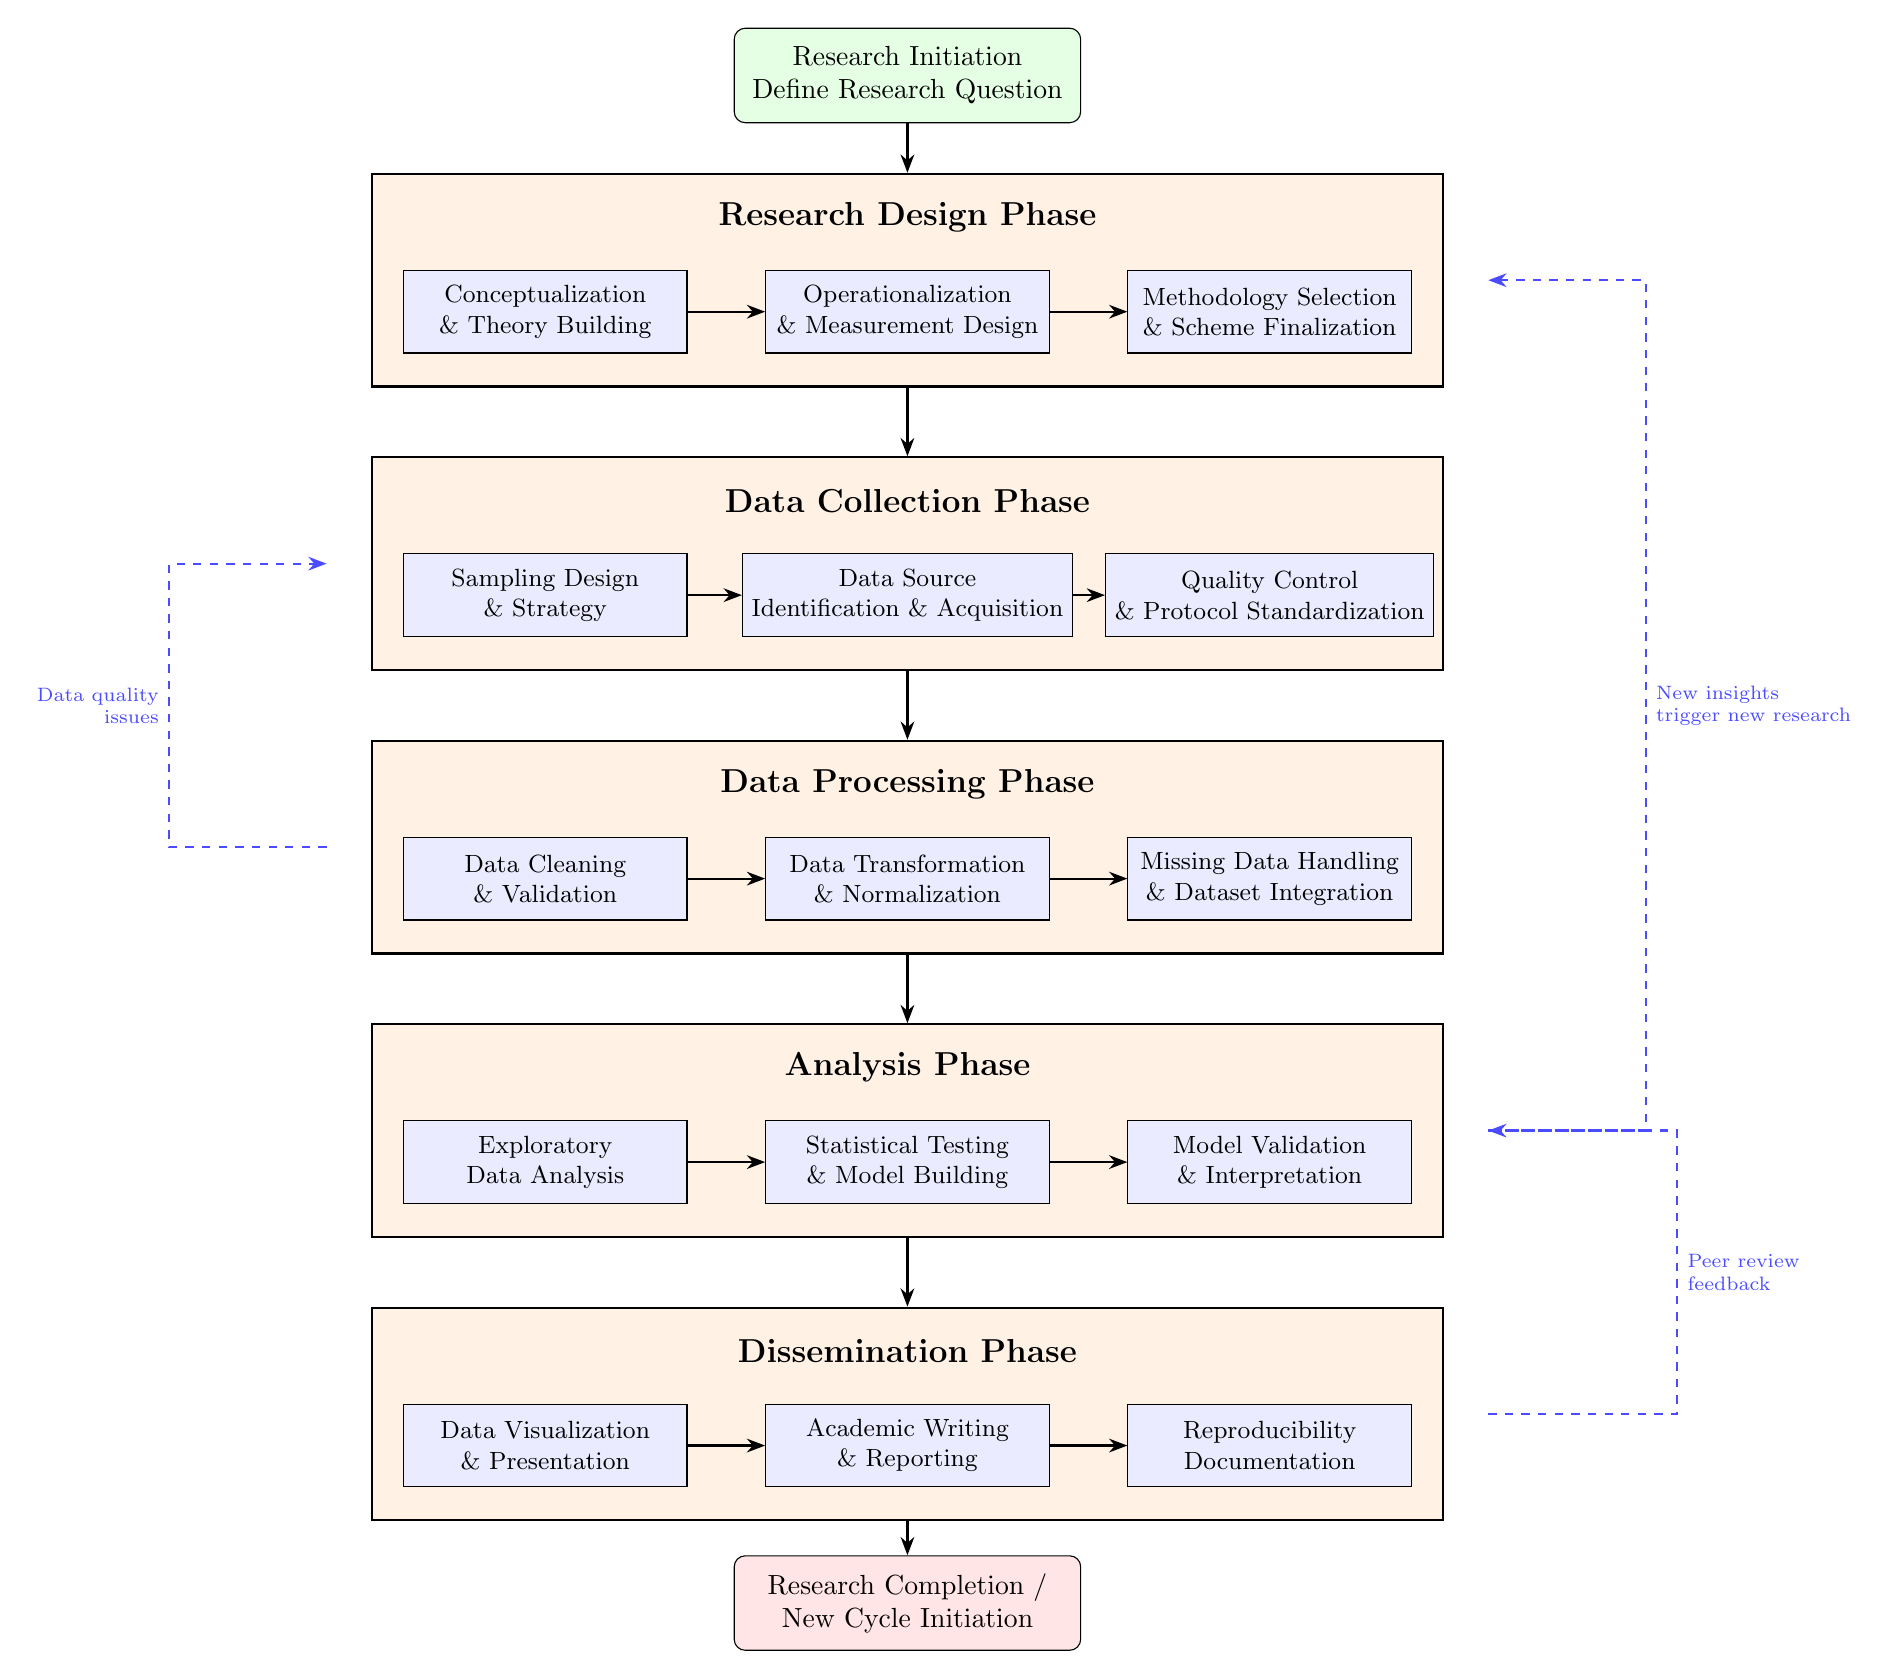
\begin{tikzpicture}[
    phasebox/.style={
        rectangle,
        minimum width=13.6cm,   minimum height=2.7cm,
        draw=black,
        thick,
        fill=orange!10
    },
    phasetext/.style={
        font=\large\bfseries,
        align=center
    },
    subtask/.style={
        rectangle,
        minimum width=3.6cm,    minimum height=1.05cm,
        align=center,
        draw=black,
        fill=blue!8,
        font=\small
    },
    mainarrow/.style={thick, ->, >=Stealth},
    feedback/.style={thick, ->, >=Stealth, dashed, blue!70, font=\scriptsize}
]

\node[phasebox] (designbox) at (0,0) {};
\node[phasetext] at (0,0.8) {Research Design Phase}; 

\node[subtask] (design1) at (-4.6, -0.4) {Conceptualization\\\& Theory Building};
\node[subtask] (design2) at (0,    -0.4) {Operationalization\\\& Measurement Design};
\node[subtask] (design3) at ( 4.6, -0.4) {Methodology Selection\\\& Scheme Finalization};

\draw[mainarrow] (design1.east) -- (design2.west);
\draw[mainarrow] (design2.east) -- (design3.west);

\node[phasebox] (collectbox) at (0,-3.6) {};
\node[phasetext] at (0,-2.8) {Data Collection Phase};

\node[subtask] (collect1) at (-4.6, -4.0) {Sampling Design\\\& Strategy};
\node[subtask] (collect2) at (0,    -4.0) {Data Source\\Identification \& Acquisition};
\node[subtask] (collect3) at ( 4.6, -4.0) {Quality Control\\\& Protocol Standardization};

\draw[mainarrow] (collect1.east) -- (collect2.west);
\draw[mainarrow] (collect2.east) -- (collect3.west);

\node[phasebox] (processbox) at (0,-7.2) {};
\node[phasetext] at (0,-6.4) {Data Processing Phase};

\node[subtask] (process1) at (-4.6, -7.6) {Data Cleaning\\\& Validation};
\node[subtask] (process2) at (0,    -7.6) {Data Transformation\\\& Normalization};
\node[subtask] (process3) at ( 4.6, -7.6) {Missing Data Handling\\\& Dataset Integration};

\draw[mainarrow] (process1.east) -- (process2.west);
\draw[mainarrow] (process2.east) -- (process3.west);

\node[phasebox] (analyzebox) at (0,-10.8) {};
\node[phasetext] at (0,-10.0) {Analysis Phase};

\node[subtask] (analyze1) at (-4.6, -11.2) {Exploratory\\Data Analysis};
\node[subtask] (analyze2) at (0,    -11.2) {Statistical Testing\\\& Model Building};
\node[subtask] (analyze3) at ( 4.6, -11.2) {Model Validation\\\& Interpretation};

\draw[mainarrow] (analyze1.east) -- (analyze2.west);
\draw[mainarrow] (analyze2.east) -- (analyze3.west);

\node[phasebox] (disseminatebox) at (0,-14.4) {};
\node[phasetext] at (0,-13.6) {Dissemination Phase};

\node[subtask] (disseminate1) at (-4.6, -14.8) {Data Visualization\\\& Presentation};
\node[subtask] (disseminate2) at (0,    -14.8) {Academic Writing\\\& Reporting};
\node[subtask] (disseminate3) at ( 4.6, -14.8) {Reproducibility\\Documentation};

\draw[mainarrow] (disseminate1.east) -- (disseminate2.west);
\draw[mainarrow] (disseminate2.east) -- (disseminate3.west);

\node[rectangle, minimum width=4.4cm, minimum height=1.2cm,
      draw=black, fill=green!10, rounded corners, align=center]
    (start) at (0, 2.6) {Research Initiation\\Define Research Question}; 

\node[rectangle, minimum width=4.4cm, minimum height=1.2cm,
      draw=black, fill=red!10, rounded corners, align=center]
    (end) at (0, -16.8) {Research Completion /\\New Cycle Initiation}; 

\draw[mainarrow] (start.south) -- (designbox.north);
\draw[mainarrow] (designbox.south) -- (collectbox.north);
\draw[mainarrow] (collectbox.south) -- (processbox.north);
\draw[mainarrow] (processbox.south) -- (analyzebox.north);
\draw[mainarrow] (analyzebox.south) -- (disseminatebox.north);
\draw[mainarrow] (disseminatebox.south) -- (end.north);

\draw[feedback]
    ([xshift=16pt]analyzebox.east) -- ++(2.0,0) |- ([xshift=16pt]designbox.east)
    node[pos=0.25, right, align=left] {New insights\\trigger new research};

\draw[feedback]
    ([xshift=-16pt]processbox.west) -- ++(-2.0,0) |- ([xshift=-16pt]collectbox.west)
    node[pos=0.25, left, align=right] {Data quality\\issues};

\draw[feedback]
    ([xshift=16pt]disseminatebox.east) -- ++(2.4,0) |- ([xshift=16pt]analyzebox.east)
    node[pos=0.25, right, align=left] {Peer review\\feedback};

\end{tikzpicture}}
\caption{Quantitative Social Science Research Lifecycle and Iterative Workflow}
\label{fig:research_workflow}
\end{figure} 
This section provides a systematic overview of quantitative social science research to establish the foundational requirements for
 our computational framework. 
We begin by describing the general research lifecycle common to most quantitative studies, 
then detail the major research schemes employed in the field, followed by an examination of analytical methods and 
dissemination practices. Throughout, we identify computational support needs that inform our computational framework design.



\subsection{Overview of Quantitative Social Science Research Lifecycle}
\label{sec:lifecycle}

Quantitative social science research is typically understood as a structured and iterative research process consisting of multiple interconnected 
stages that interact and provide 
feedback to one another in research practice~\cite{grinnell2019practice, creswell2017research}.

In this paper, we conceptualize this research process as a research lifecycle comprising five core stages, and explicitly incorporate problem discovery 
as the first stage of the research lifecycle. This delineation is made because the problem discovery stage plays a critical role in research practice by 
establishing the research context, motivation, and formalizing research objectives, which will constrain all subsequent research design, data processing, 
and analytical activities.

Understanding this complete research lifecycle is fundamentally important for designing computational tools that can support the entire research process.
Figure \ref{fig:research_workflow} illustrates the relationships among the various stages in the research lifecycle, as well as the key constituent elements of each stage.

In the research design stage, researchers need to identify and define theoretical concepts relevant to the research question. This process is typically accomplished through 
developing or adopting existing theoretical frameworks. Due to the highly abstract nature of theoretical concepts, subsequent quantitative 
analysis requires an operationalization process to transform these abstract concepts into measurable and observable variables~\cite{adcock2001measurement}. Building upon this
 foundation, researchers further design research protocols for data collection, including measurement instruments, sampling strategies, and data acquisition methods.
 
 In the data collection stage, researchers implement the acquisition of empirical data according to the established research design. This process typically 
 requires selecting appropriate sampling methods and data collection strategies based on the target characteristics of the research task and resource and 
 contextual constraints under real-world conditions. Researchers need to determine specific data sources and conduct actual data collection activities such 
 as questionnaire surveys, experiments, observations, or archival data extraction. This stage often also includes quality control and process standardization to 
 ensure consistency of data across different time points, locations, 
 or personnel~\cite{fowler2013survey}.
 
 The objective of the data processing stage is to prepare appropriate data representations for subsequent analysis. Researchers typically need to clean, 
 transform, and integrate raw data to address issues such as noise, outliers, missing data, and inconsistent data structures~\cite{little2019statistical}. 
 When research involves multiple data types, or even multimodal data, data integration procedures are also required to merge data from different sources into 
 a consistent analytical dataset.
 
 In the data analysis stage, researchers employ various methodological frameworks to extract research findings from the processed data. Modern quantitative social science, 
 beyond traditional statistical methods, extensively adopts analytical frameworks such as machine learning methods, information-theoretic approaches, graph-theoretic models, 
 and systems theory~\cite{breiman2001statistical, watts1998collective}. This stage typically includes exploratory data analysis, modeling and validation, and 
 interpretation of analytical results within the theoretical context.
 
 The final stage of the research lifecycle is the dissemination stage. In this stage, researchers communicate research findings through various forms such as papers, 
 reports, and conference presentations, combining text, visualizations, and other media to suit different audiences~\cite{brownson2018dissemination}. 
 This stage also typically includes systematic documentation and organization of the research process and analytical results, such as making data, code, and methodological 
 descriptions publicly available, to support verification and reuse of research results~\cite{gentzkow2014code}.
 
These five stages together constitute an iterative research process characterized by feedback loops and stage-to-stage interaction.
 Findings from subsequent stages often prompt 
 researchers to return to earlier stages to revise the research question, research design, or data processing strategies. For example, the analysis stage may reveal deficiencies
  in data collection, preliminary results may trigger theoretical reconsideration, and feedback obtained during the dissemination process may also generate new research questions. 
  This iterative characteristic highlights the importance of maintaining coherence across stages and consistency of research products throughout the entire research lifecycle.


\subsection{Methodologies of Quantitative Social Science Research Lifecycle}
\subsubsection{Question Discovery}

Problem discovery constitutes a foundational stage in quantitative social science research, serving as the prerequisite for subsequent methodological and analytical decisions.
 From a methodological perspective, this stage primarily involves two fundamental questions: how 
research questions are generated, and how to judge whether a research question merits further investigation.

Relevant methodological literature indicates that research questions may originate from researchers' observations of social reality, personal or professional experiences, and 
systematic reading of existing research literature~\cite{feng2018socialmethods}. These sources are typically integrated through the researcher's theoretical imagination 
and methodological judgment. Existing research has also proposed a series of criteria for evaluating research questions, including importance, originality, feasibility, and 
appropriateness.

Among these, importance reflects the potential value of the research question at the levels of theoretical contribution and social significance; originality 
focuses on its degree of novelty relative to existing research; feasibility concerns whether the research question can be systematically addressed under existing theories, 
methods, and real-world conditions; appropriateness reflects the degree of alignment between the research question and the researcher's own background, professional 
capabilities, and available resources.

These considerations indicate that before formally entering quantitative analysis, researchers typically need to invest substantial intellectual 
and methodological 
work. Problem discovery is therefore an active, creative, and evaluative stage that largely shapes the scope, direction, and 
feasibility of the entire research lifecycle.


\subsubsection{Research Design Phase}
The core task of the research design stage is to transform the research question into an implementable research protocol. 
In this stage, researchers first need to clarify the research subjects and units of analysis, and formulate the research question formally so that 
it can be answered through empirical data. This process is typically based on a systematic literature review, which is used to identify relevant theoretical frameworks, existing 
research conclusions, and methodological approaches that can be drawn upon.

A key component of the research design stage is variable identification and operationalization. Researchers need to identify core concepts involved in 
the research question and transform abstract concepts into measurable variables or indicators through the operationalization process. Operationalization methods may include adopting 
existing scales, constructing new measurement indicators, or mapping theoretical concepts to observable objects such as behavioral frequencies, attitude ratings, structural 
characteristics, or event occurrence patterns. In this process, researchers need to address issues such as construct validity, content validity, and measurement reliability.

After variables are clarified, researchers typically formulate research hypotheses based on theoretical derivation, explicitly specifying the expected relationships 
among variables in a testable form. 
Research may pursue hypothesis testing or exploratory objectives; in both cases, preliminary conceptions of variable relationships help guide subsequent research design.

The research design stage also includes the selection and planning of research schemes. Common schemes include questionnaire survey research, experimental or 
quasi-experimental research, secondary data analysis, literature and text analysis, comparative research, and mixed-methods research, among others. 
Different schemes differ significantly in data sources, sample structure, inference approaches, and applicable question types. With the development of computational 
methods, some research also adopts more complex design forms, such as nested designs, multilevel designs, or integrated research protocols combining multiple data sources.

Additionally, researchers need to conduct overall planning at this stage for sampling strategies, measurement instruments, data collection procedures, 
and preliminary analytical methods. These decisions collectively constitute the blueprint for research implementation and directly impact the feasibility 
and research quality of subsequent stages.

\subsubsection{Data Collection Phase}
The data collection stage transforms the research design into concrete empirical data. In this stage, researchers need to select appropriate sampling methods 
according to the research protocol to ensure sample representativeness of the target population as much as possible under resource constraints. Probability 
sampling methods (such as simple random sampling, stratified sampling, cluster sampling, and multistage sampling) provide the foundation 
for statistical inference, while nonprobability sampling methods (such as convenience sampling, purposive sampling, quota sampling, and snowball sampling) are 
commonly used for exploratory research or hard-to-reach research populations.

In the actual data collection process, researchers need to attend to various potential sampling biases and systematic errors, such as coverage bias, 
nonresponse bias, self-selection bias, and measurement error. Some research also employs methods such as weighting adjustments, post-stratification, or sensitivity analysis 
to quantitatively assess and correct sampling errors.

The choice of data sources depends on the research protocol and may include questionnaire platforms, experimental facilities, archival data, administrative 
records, network interfaces, or sensor systems, among others. The data collection process typically needs to be controlled through standardized procedures, 
accompanied by quality control measures such as pretesting, real-time validation, and data auditing to reduce human errors and systematic biases.

Additionally, the data collection stage requires detailed documentation of the data acquisition process, including sampling decisions, implementation deviations, and field 
conditions, to support subsequent data interpretation and reproducibility assessment.




\subsubsection{Data Processing Phase}
The objective of the data processing stage is to transform raw data into data representations suitable for systematic analysis while controlling information loss 
and structural biases introduced during the processing as much as possible. Researchers typically begin with data cleaning and validation, including correcting entry 
errors, identifying outliers, handling logical inconsistencies, and verifying whether variable values fall within reasonable ranges~\cite{van2018flexible}. 
These operations, while procedural in form, often exert substantial influence on subsequent analytical results.

Missing data handling is an important component of the data processing stage~\cite{little2019statistical}. Researchers need not only to identify the proportion and distribution of missing data 
but also to analyze its underlying mechanisms and select appropriate handling methods accordingly. 
Different handling strategies involve trade-offs between bias reduction and information retention, with implications for effective sample size and data integrity.

In the process of variable transformation and recoding, information loss control is likewise a key consideration. Discretization of continuous variables, 
aggregation of time series, simplified representations of text data, and threshold processing of network structures may all sacrifice fine-grained information while improving 
computational feasibility. Researchers typically need to balance interpretability, computational complexity, and information retention, and when necessary, preserve raw 
data or intermediate representations to support sensitivity analysis~\cite{wickham2016r}.

When research involves multi-source or multimodal data, the data integration process may introduce additional information loss risks, such as temporal 
asynchrony, inconsistent measurement scales, or semantic mismatches. To mitigate these risks, researchers employ various alignment strategies. For instance, when integrating survey data 
with administrative records, researchers may use temporal alignment by matching records by date ranges or event sequences, and semantic mapping by standardizing occupation codes or geographic 
classifications across different coding systems~\cite{harron2017guide}. Metadata management throughout the integration process helps document transformation decisions and ensures traceability. 
Consistency assessments compare overlapping measurements from different sources or validate integrated variables against known benchmarks to help identify potential integration errors.

Furthermore, in research involving high-dimensional data, unstructured data, or privacy-sensitive data, the data processing stage may include complex 
operations such as dimensionality reduction, feature extraction, structural reconstruction, or anonymization. Common dimensionality reduction techniques include 
\textit{principal component analysis} and \textit{factor analysis}~\cite{jolliffe2016principal}. Feature extraction may involve generating text embeddings~\cite{mikolov2013efficient} or 
extracting image features~\cite{krizhevsky2012imagenet}. 
Structural reconstruction includes network inference from behavioral data~\cite{newman2018networks}. Anonymization approaches include \textit{k-anonymity}~\cite{sweeney2002k} 
and \textit{differential privacy} mechanisms~\cite{dwork2014algorithmic}. While these operations improve analytical 
feasibility, they often involve irreversible information compression and therefore require clarification of their potential impacts on research conclusions 
through method selection, parameter control, and robustness testing.

\subsubsection{Data Analysis Phase}
The data analysis stage aims to extract empirical findings that can answer research questions from processed data through systematic analytical methods. 
This stage typically begins with exploratory data analysis, which uses descriptive statistics, data visualization, and pattern recognition to help researchers understand data 
structure, variable distributions, and potential associational relationships, providing a basis for subsequent modeling~\cite{tukey1977exploratory}.

In inferential analysis, researchers commonly employ statistical modeling methods to characterize relationships among variables. Regression analysis 
is widely used to estimate the strength and direction of associations among variables, with specific forms including \textit{ordinary least squares regression}, \textit{logistic regression}, 
\textit{Poisson regression}, \textit{generalized linear models}~\cite{nelder1972generalized}, \textit{generalized additive models}~\cite{hastie1990generalized}, and \textit{multilevel models} or \textit{hierarchical models} for nested data structures~\cite{raudenbush2002hierarchical}. Beyond simple bivariate or 
multivariate associations, researchers often need to analyze more complex effect structures. \textit{Mediation analysis} examines whether and how an independent variable affects 
a dependent variable through intermediate mechanisms, estimating both direct and indirect effects~\cite{baron1986moderator, imai2010general}. \textit{Moderation analysis}, also known as \textit{interaction analysis}, investigates 
whether the relationship between variables varies across levels of a third variable, identifying conditional effects and boundary conditions~\cite{aiken1991multiple}. Some research also employs 
\textit{moderated mediation} or \textit{mediated moderation} models to characterize even more complex theoretical relationships~\cite{preacher2007addressing}.

In causal analysis contexts, researchers may employ various identification strategies to isolate causal effects under observational data conditions. \textit{Difference-in-differences} 
methods compare changes over time between treatment and control groups to account for time-invariant confounders~\cite{angrist2009mostly}. \textit{Instrumental variable methods} use exogenous variables that affect the treatment 
but not the outcome directly to address endogeneity bias~\cite{angrist1996identification}. \textit{Propensity score methods}, including matching, weighting, and stratification, balance treatment and control groups 
on observed covariates~\cite{rosenbaum1983central}. \textit{Regression discontinuity designs} exploit threshold-based treatment assignment rules~\cite{imbens2008regression}. \textit{Synthetic control methods} construct counterfactual comparisons 
by combining control units~\cite{abadie2010synthetic}. Panel data methods, such as \textit{fixed effects models} and \textit{first-difference models}, control for time-invariant unobserved heterogeneity~\cite{wooldridge2010econometric}.

With the development of computational social science, machine learning methods have been widely introduced in the data analysis stage~\cite{breiman2001statistical, mullainathan2017machine}. Supervised learning methods 
are used for predictive modeling and classification tasks, including \textit{decision trees}, \textit{random forests}~\cite{breiman2001random}, \textit{gradient boosting machines}~\cite{friedman2001greedy}, \textit{support vector machines}~\cite{cortes1995support}, \textit{neural networks}, and \textit{deep learning models}~\cite{lecun2015deep}. Unsupervised learning methods help discover latent patterns and structures in data, including \textit{k-means clustering}, \textit{hierarchical clustering}, \textit{Gaussian mixture models}, and dimensionality reduction 
techniques such as \textit{principal component analysis}, \textit{t-SNE}~\cite{maaten2008visualizing}, and \textit{UMAP}~\cite{mcinnes2018umap}. \textit{Ensemble methods} combine multiple models to 
improve predictive performance~\cite{dietterich2000ensemble}. 
These methods typically emphasize predictive accuracy, which calls for careful alignment with research objectives regarding interpretability and inference.

In contexts where research subjects possess relational or interactive structures, network analysis methods model and analyze nodes, edges, 
and overall structural characteristics~\cite{wasserman1994social, newman2018networks}. Centrality measures characterize 
node importance, including \textit{degree centrality}, \textit{betweenness centrality}, \textit{closeness centrality}, and \textit{eigenvector centrality}~\cite{freeman1978centrality}. Community detection algorithms identify cohesive 
subgroups through approaches such as \textit{modularity optimization}~\cite{newman2006modularity}, \textit{spectral clustering}~\cite{von2007tutorial}, and \textit{stochastic block models}~\cite{holland1983stochastic}. \textit{Network motifs}~\cite{milo2002network} and \textit{graphlets}~\cite{przulj2007biological} characterize local structural patterns. \textit{Exponential random graph models} (ERGMs)~\cite{lusher2013exponential} and \textit{stochastic actor-oriented models} (SAOMs)~\cite{snijders2010introduction} enable 
statistical inference about network formation processes. Dynamic network models capture temporal evolution of relational structures, including discrete-time 
and continuous-time approaches~\cite{holme2012temporal}.

For temporally related data, time series analysis methods study patterns of variable changes over time. \textit{Autoregressive models}, \textit{moving average 
models}, and \textit{autoregressive integrated moving average (ARIMA) models} capture temporal dependencies~\cite{box2015time}. \textit{State-space models} and \textit{structural time series 
models} decompose temporal patterns into trends, seasonal components, and irregular fluctuations~\cite{durbin2012time}. \textit{Vector autoregression (VAR) models} analyze multivariate 
time series systems~\cite{lutkepohl2005new}. \textit{Event history analysis}, also known as \textit{survival analysis} or \textit{duration analysis}, examines time-to-event processes using methods 
such as \textit{Kaplan-Meier estimation}, \textit{Cox proportional hazards models}, and parametric survival models~\cite{cox1972regression, allison2014event}.

Beyond the above methods, some research employs information-theoretic methods to analyze uncertainty, information transfer, and structural complexity. \textit{Shannon entropy} measures 
uncertainty in probability distributions~\cite{shannon1948mathematical}. \textit{Mutual information} quantifies statistical dependencies between variables without assuming functional forms~\cite{cover1999elements}. \textit{Transfer entropy}~\cite{schreiber2000measuring} and \textit{Granger 
causality}~\cite{granger1969investigating} assess directional information flow in temporal or spatial systems. Complexity measures, such as \textit{Kolmogorov complexity} and \textit{algorithmic information theory}, characterize 
structural regularity and randomness~\cite{li2008introduction}. These methods are particularly useful in analyzing high-dimensional, multivariate, or dynamical systems where traditional parametric 
assumptions may be overly restrictive.

In research involving explicit theoretical structures, researchers may also introduce domain-specific structural models that directly embed theoretical assumptions into 
model structures. \textit{Agent-based models} simulate individual-level decision rules and emergent collective patterns~\cite{epstein1996growing, railsback2011agent}. \textit{Compartmental models}, such as \textit{SIR models} in epidemiology, 
represent flow between discrete states~\cite{kermack1927contribution}. \textit{System dynamics models} use differential equations to represent feedback loops and stock-flow relationships~\cite{forrester1961industrial, sterman2000business}. These structured modeling 
approaches enable researchers to formalize theoretical mechanisms and explore implications of different theoretical assumptions through simulation and analytical derivation.

Regardless of which analytical method is employed, model validation and robustness testing are important components of the data analysis stage. Researchers typically 
assess the stability and generalizability of results through \textit{cross-validation}, \textit{out-of-sample testing}, alternative model comparison, parameter sensitivity analysis, or 
subsample analysis~\cite{hastie2009elements}. For causal inference, researchers conduct \textit{placebo tests}, \textit{falsification tests}, and sensitivity analyses for unobserved confounding~\cite{rosenbaum2002observational, imbens2015causal}. 
The interpretation of analytical results needs to be combined with theoretical background, clarifying the applicable scope of model assumptions, and carefully 
distinguishing among statistical correlation, predictive capability, and causal interpretation.




















\subsubsection{Dissemination Phase}
\label{sec:dissemination_phase}

The dissemination stage transforms research findings into forms that enable academic and social impact. The primary objective is to communicate research contributions to 
appropriate audiences while ensuring transparency and reproducibility of the research process.

Academic journal publication establishes formal scholarly records and enables peer review for quality assurance. Journal articles typically follow discipline-specific conventions 
in presenting research questions, theoretical frameworks, methods, results, and implications. Researchers select journals based on fit with their research topic, 
methodological approach, and target readership. The peer review process provides critical feedback and validation of research quality.

Conference presentations enable rapid knowledge exchange and direct engagement with research communities. Academic conferences provide opportunities for early-stage feedback, 
networking, and staying current with emerging research directions. Presentation formats include oral presentations, poster sessions, and panel discussions, each suited to different 
types of content and interaction goals.

Preprint releases accelerate scientific communication by making research publicly available before formal peer review. Preprint repositories such as 
arXiv~\footnote{https://arxiv.org}, SSRN~\footnote{https://www.ssrn.com}, and SocArXiv~\footnote{https://osf.io/preprints/socarxiv} establish priority claims while enabling broader 
access. This approach is particularly valuable for rapidly evolving research areas or when timely dissemination serves public interest.

Policy briefs and stakeholder reports translate research findings into accessible formats for decision-makers and practitioners. These communications emphasize actionable implications 
while maintaining scientific integrity. Effective policy communication requires adapting technical content to non-specialist audiences, highlighting practical relevance, and 
acknowledging limitations and uncertainties.

Public communication activities, including media engagement, public lectures, and educational outreach, broaden research impact beyond academic communities. These 
activities fulfill accountability to funding sources and society while contributing to public understanding of social science research.

Contemporary dissemination increasingly integrates open science practices. Data sharing through repositories such as 
ICPSR~\footnote{https://www.icpsr.umich.edu}, Dataverse~\footnote{https://dataverse.org}, and OSF~\footnote{https://osf.io} enables verification and secondary analysis. 
Code sharing through platforms such as GitHub~\footnote{https://github.com} and GitLab~\footnote{https://gitlab.com} documents analytical procedures and supports computational 
reproducibility. Computational environment documentation through tools such as Docker~\footnote{https://www.docker.com} preserves the complete software stack. 
Detailed methodological documentation, including protocols, instruments, and decision logs, supports replication and extension of research.

These various dissemination forms serve complementary functions in the research ecosystem. Feedback obtained during dissemination often reveals new questions, 
methodological refinements, or directions for improvement, thereby driving new research cycles. The choice among dissemination strategies depends on research objectives, 
target audiences, institutional requirements, and available resources. \subsection{Research Schemes in Quantitative Social Science}

Research schemes in this work are comprehensive approaches that structure the entire research process from problem 
formulation through data collection to analysis and interpretation~\cite{creswell2017research}. 
Each scheme represents a distinct way of conducting social science inquiry and can employ multiple specific analytical methods. 
The choice of research scheme depends on the research question, theoretical framework, available resources, and epistemological commitments. 
Below we describe the major research schemes in quantitative social science, emphasizing their distinct 
workflows and computational support needs.

\subsubsection{Literature Review and Meta-Analysis}

Systematic literature reviews and meta-analyses synthesize existing research to identify patterns, gaps, and theoretical 
frameworks~\cite{cooper2015research}.
Systematic literature reviews employ explicit, reproducible methods for searching, screening, and synthesizing literature, distinguishing them from narrative review approaches.
Meta-analysis extends systematic review by quantitatively combining effect sizes across 
studies to estimate overall effects with greater precision than individual studies can provide~\cite{borenstein2021introduction}.

As a research scheme in quantitative social science, the literature review lifecycle begins with question discovery, 
followed by research design or planning, as indicated in Section~\ref{sec:lifecycle}. It should be noted that researchers may 
define new specific research questions beyond the initial ones during the review process. They also establish clear inclusion and exclusion 
criteria, often using frameworks such as PICO representing Population, Intervention, Comparison, and Outcome, 
and develop a priori protocols to 
minimize bias~\cite{page2021prisma}. Search strategies must be comprehensive and reproducible, specifying keywords, Boolean operators, 
database selections, and search syntax. Advanced techniques include citation chaining and hand-searching key journals. Screening proceeds 
in stages, beginning with title and abstract review to identify potentially relevant studies, followed by 
full-text review applying detailed eligibility criteria. Multiple independent reviewers typically conduct screening to ensure 
reliability.

Data extraction involves systematically coding study characteristics such as design, sample, and setting, along with methods 
including measurement and analysis, and findings covering effect sizes, confidence intervals, and p-values. 
Standardized extraction forms and codebooks ensure consistency across reviewers. Quality assessment evaluates methodological rigor and risk 
of bias using validated instruments like the Cochrane Risk of Bias tool or GRADE framework. 
Synthesis can be narrative, qualitatively describing patterns across studies, or quantitative, 
involving meta-analysis through effect size aggregation, meta-regression for moderator analysis, and publication bias 
assessment via funnel plots and statistical tests. Interpretation draws conclusions about the state of knowledge, identifies theoretical 
and empirical gaps, and provides recommendations for future research. Finally, reporting follows established guidelines such as 
\textit{PRISMA} or \textit{MOOSE} to ensure transparency and reproducibility.

Literature reviews employ diverse analytical methods beyond simple narrative synthesis. 
Descriptive statistics summarize study characteristics and sample demographics. Effect size calculation standardizes findings across studies using 
metrics like Cohen's d, odds ratios, or correlation coefficients. Meta-regression examines how study characteristics moderate effects, while
 subgroup analysis compares effects across predefined categories. Publication bias assessment utilizes funnel plots, Egger's test, 
 trim-and-fill methods, and p-curve analysis. More recently, citation network analysis maps intellectual structures and identifies influential works, 
 and topic modeling using techniques like \textit{Latent Dirichlet Allocation} or \textit{BERTopic} can identify thematic patterns 
 across large literature corpora.

However, researchers conducting systematic reviews face substantial challenges. Information overload continues to worsen 
as scholarly production accelerates. Selection bias can occur if search strategies miss relevant studies 
or if eligibility criteria inadvertently exclude important work. Publication bias, which favors statistically 
significant findings, potentially distorts meta-analytic estimates. Cross-database redundancy requires careful 
deduplication to avoid counting the same study multiple times. Heterogeneity in study designs, populations, and 
measures complicates synthesis and limits the applicability of pooled estimates. The time and resource intensity 
of comprehensive reviews makes them challenging for individual researchers to complete without substantial support.

These challenges create clear computational support needs. Effective tools for literature reviews require automated 
search across multiple databases with unified query interfaces, intelligent duplicate detection using fuzzy matching 
and DOI resolution, AI-assisted screening to accelerate title and abstract review while maintaining accuracy, 
citation network analysis tools to identify seminal works and research communities, and statistical meta-analysis 
software implementing fixed-effect, random-effects, and mixed-effects models. Advanced features might include 
automated data extraction from PDFs, inter-rater reliability calculators, and seamless integration with reference 
management systems. Visualization tools such as PRISMA flow diagrams are also essential for documenting the screening process.

\subsubsection{Experimental Research}
Experimental research establishes causal relationships through controlled manipulation of independent variables 
while observing effects on dependent variables~\cite{shadish2002experimental}. This paradigm emphasizes internal validity through 
experimental control, randomization, and comparison groups, providing the strongest evidence for causality by isolating treatment effects 
from confounding variables.

Experimental design requires selecting an appropriate experiment structure. 
\textit{Randomized controlled trials}, abbreviated as RCTs, randomly assign participants to treatment and control conditions, 
establishing the gold standard for causal inference. \textit{Quasi-experiments} lack randomization but employ techniques like matching, 
regression discontinuity, or difference-in-differences to approximate experimental conditions when randomization is 
infeasible~\cite{cook2002experimental}. 
\textit{Factorial designs} manipulate multiple factors simultaneously to examine main effects and interactions. \textit{Repeated measures designs} reduce error 
variance by using participants as their own controls.
Planning involves power analysis to determine required sample sizes for detecting effects of theoretical interest~\cite{cohen1988statistical}, 
developing detailed randomization procedures including simple, block, stratified, or adaptive randomization, and preparing standardized treatment protocols. 
Implementation requires careful treatment assignment, intervention delivery with fidelity monitoring, appropriate control group management including placebo controls, and 
blinding procedures to prevent expectancy effects. Measurement includes pre-treatment baseline assessments, manipulation checks to verify treatment mechanisms, and 
continuous outcome monitoring with quality control.

Beyond simple treatment effect estimation, experimental research employs sophisticated statistical methods for understanding 
causal mechanisms—techniques valuable across all research paradigms, not merely experiments. \textit{Mediation analysis} examines 
indirect effects through which independent variables influence outcomes via intermediate variables~\cite{baron1986moderator}. 
For instance, a stress reduction intervention may improve academic performance through decreased anxiety as a mediating mechanism. \textit{Moderation analysis} identifies 
conditions under which treatment effects vary, revealing for whom or under what circumstances interventions work best. Adjustment methods control for confounding 
variables that may bias treatment effect estimates, using 
techniques like ANCOVA, propensity score matching~\cite{rosenbaum1983central}, or inverse probability weighting. \textit{Interaction effect analysis} explores synergistic 
or antagonistic combinations of multiple factors. \textit{Difference-in-differences estimators} leverage pre-post comparisons across treatment and control groups to isolate 
causal effects~\cite{angrist2008mostly}. \textit{Instrumental variable methods} address unmeasured confounding when natural experiments or randomization encourage but do not 
determine treatment assignment. \textit{Regression discontinuity designs} exploit threshold-based treatment assignment to estimate local average treatment effects. These causal 
analysis frameworks, while particularly powerful in experimental contexts, extend to observational, survey, and qualitative research paradigms when appropriate assumptions hold.

The primary difficulty in experimental research lies in designing studies that adequately represent real-world complexity 
while maintaining experimental control. Researchers must navigate numerous interacting factors that can influence results. 
Trade-offs between internal validity referring to control and precision and external validity referring to generalizability require careful 
consideration~\cite{shadish2002experimental}—highly controlled laboratory settings may not reflect messy real-world conditions. 
Ethical constraints limit permissible manipulations, particularly with vulnerable populations. Participant attrition threatens 
validity if dropout patterns differ between conditions or correlate with outcomes. Contamination occurs when control group 
participants receive treatment elements through communication or diffusion. Despite randomization, confounding may persist 
in small samples or when randomization fails to balance unmeasured variables. Hawthorne effects cause behavioral changes 
from participants' awareness of being studied. Demand characteristics lead participants to infer study hypotheses and alter 
responses accordingly. Treatment fidelity varies when interventions cannot be delivered uniformly across sites or providers. 
Temporal factors like maturation, history effects, or regression to the mean complicate causal inference. Measurement 
reactivity occurs when repeated assessments themselves influence outcomes. Complex interactions between individual 
characteristics, contextual factors, and treatment components may require large samples and sophisticated designs 
to detect. Longitudinal experiments face compounding challenges as time-varying confounders and dynamic treatment 
regimens introduce additional complexity.

Computational tools support experimental research through randomization algorithms implementing various allocation 
schemes such as simple, block, stratified, or minimization methods, power analysis calculators for 
sample size determination considering effect sizes and statistical tests, causal inference estimation 
methods such as propensity scores, instrumental variables, or regression discontinuity approaches, mediation and moderation 
analysis frameworks, treatment effect visualization with uncertainty quantification, and compliance 
tracking systems monitoring adherence and protocol deviations.

\subsubsection{Survey Research}
Survey research gathers systematic primary data from populations through structured data collection instruments to describe characteristics, 
attitudes, behaviors, or relationships~\cite{groves2009survey}. This scheme emphasizes representativeness through probability 
sampling and generalizability through statistical inference. Surveys efficiently collect standardized data from large samples, 
enabling population estimates and examination of associations between variables.

Survey designs can be classified along multiple dimensions. By temporal structure, \textit{cross-sectional surveys} collect data at a single time point, 
providing a snapshot of population characteristics but precluding causal inference about change. \textit{Longitudinal surveys} involve repeated measurements over time, enabling 
analysis of temporal patterns, trends, and causal processes. Longitudinal designs include \textit{trend studies}, which sample different individuals from the same population 
at multiple time points to track population-level changes; \textit{cohort studies}, which follow a specific cohort such as a birth cohort or graduating class through repeated 
measurements to examine life course trajectories; and \textit{panel studies}, which repeatedly survey the same individuals, providing the strongest design for analyzing 
individual-level change and within-person dynamics~\cite{lynn2009methodology}. Panel studies enable growth curve modeling, fixed effects estimation, and dynamic causal analysis, 
though they face challenges from panel attrition and conditioning effects from repeated measurement.

Survey data collection has evolved substantially beyond traditional questionnaires to encompass diverse instruments and modalities. Traditional approaches 
include \textit{structured questionnaires} administered via paper, web, or mobile platforms, and \textit{structured interviews} conducted through telephone, 
face-to-face, or video formats. Contemporary technological developments have expanded data collection possibilities. \textit{Ecological momentary assessment}, abbreviated 
as EMA, uses smartphones to collect real-time data in naturalistic settings, reducing recall bias~\cite{shiffman2008ecological}. \textit{Wearable devices and sensors} including fitness 
trackers, smartwatches, and environmental sensors passively collect behavioral and physiological data when integrated into research designs with informed 
consent. \textit{Digital trace data} from social media, web browsing, or mobile applications can be collected through research partnerships or participant-authorized 
data donations~\cite{salganik2017bit}. Some survey research also incorporates linkage to \textit{administrative records} such as tax records, educational transcripts, 
or health insurance claims, or to \textit{electronic health records}, though this represents a hybrid approach between primary data collection and secondary data analysis.

It is important to distinguish survey research from secondary data analysis based on the researcher's role in data generation. Survey research involves researchers 
actively designing and implementing data collection protocols, even when leveraging digital technologies or administrative systems. The researcher determines sampling frames, 
measurement instruments, timing, and consent procedures. In contrast, secondary data analysis examines datasets originally collected for other purposes such as existing EHR systems, 
government statistics, or archived surveys. The boundary can blur when researchers design linkage studies connecting survey data to pre-existing administrative records, but 
the defining characteristic of survey research is the intentional design of primary data collection to address specific research questions.

Survey research begins with conceptualization, where researchers define 
constructs of interest and identify relevant variables. Instrument development involves crafting clear, unbiased questions, 
selecting appropriate response scales including \textit{Likert scales}, \textit{semantic differential scales}, and \textit{visual analog scales}, structuring questionnaire flow with
 attention to question order effects, and conducting cognitive interviewing to identify 
 comprehension problems~\cite{tourangeau2000psychology}. For technology-based data collection, instrument development also includes designing sensor protocols, defining event triggers 
 for EMA, or specifying data streams for passive collection. Pilot testing on small samples assesses 
 reliability including test-retest reliability and internal consistency, validity including content validity, criterion validity, and construct validity, and identifies problems with
  wording, skip patterns, or administration.

Sampling design defines the target population, selects sampling methods based on resources and research goals, 
and determines required sample sizes considering precision requirements and anticipated response
 rates~\cite{cochran1977sampling}. Probability 
 sampling methods including \textit{simple random sampling}, \textit{stratified sampling}, \textit{cluster sampling}, and \textit{multistage sampling} enable statistical inference to 
 populations, whereas non-probability methods such as \textit{convenience sampling}, \textit{purposive sampling}, \textit{quota sampling}, and \textit{snowball sampling} may be 
 appropriate when probability sampling is 
 infeasible, though they limit generalizability. For longitudinal designs, sampling must also address panel maintenance strategies, refreshment samples to address attrition, and 
 rotation patterns for repeated cross-sections.

Data collection implements surveys through various modes with distinct advantages and limitations. \textit{Online surveys} offer cost efficiency and rapid deployment but face 
coverage bias toward internet-connected populations. \textit{Mail surveys} reach diverse populations but suffer from low response rates and slow turnaround. \textit{Telephone surveys} enable 
probability sampling through random digit dialing but face declining response rates and mobile-only household challenges. \textit{Face-to-face interviews} achieve high response quality 
and can include complex tasks or biomarker collection, but require substantial resources. \textit{Mixed-mode designs} combine approaches to balance coverage, cost, and data 
quality~\cite{dillman2014internet}. For technology-based collection, researchers must address informed consent for passive data collection, data security and privacy protections, participant 
burden from frequent assessments, and technical support for device issues. Response monitoring tracks completion rates with real-time dashboards and implements follow-up procedures 
to maximize participation while minimizing nonresponse bias.

Data preparation includes data entry or import, coding of open-ended responses through manual coding or text analysis, 
and missing data handling. Validation involves reliability testing using \textit{Cronbach's alpha} for internal 
consistency~\cite{cronbach1951coefficient}, test-retest reliability for temporal stability, 
and construct validity assessment through \textit{confirmatory factor analysis}~\cite{brown2015confirmatory}. Scale refinement drops poor-performing items based on 
item-total correlations, factor loadings, and reliability improvement. Analysis includes descriptive statistics, inferential tests, and multivariate modeling. 
Interpretation generalizes findings to the population, acknowledges sampling and non-sampling errors, and considers limitations. Reporting documents sampling 
procedures, response rates, measurement properties, and weighting adjustments following standards such as AAPOR reporting guidelines.

Survey analysis employs a range of analytical methods appropriate to the research design. Descriptive statistics provide univariate and bivariate summaries, while correlation analysis examines 
linear associations between variables. Regression models estimate relationships while controlling for confounders, including \textit{linear regression} for continuous 
outcomes, \textit{logistic regression} for binary outcomes, \textit{ordinal regression} for ordered categories, and \textit{multilevel modeling} for nested 
data structures~\cite{gelman2006data}. For longitudinal data, \textit{growth curve models} and \textit{latent growth curve models} examine trajectories of change~\cite{singer2003applied}, 
\textit{fixed effects models} control for time-invariant unobserved heterogeneity, \textit{random effects models} efficiently estimate between-person and within-person effects, 
and \textit{dynamic panel models} incorporate lagged dependent variables. \textit{Factor analysis}, both exploratory and confirmatory, assesses measurement structure and construct validity. 
\textit{Structural equation modeling} simultaneously estimates measurement models and structural relationships~\cite{kline2015principles}. \textit{Cluster 
analysis} identifies homogeneous subgroups, while \textit{latent class analysis} discovers categorical latent variables~\cite{collins2009latent}. Text mining analyzes open-ended 
responses using sentiment analysis, topic modeling, or word 
frequencies. Weighting procedures adjust for unequal selection probabilities, nonresponse, and coverage error to improve population representativeness through techniques 
such as \textit{raking}, \textit{post-stratification}, and \textit{calibration weighting}. 
Missing data imputation techniques including \textit{multiple imputation} and \textit{maximum likelihood estimation} address item nonresponse~\cite{little2019statistical}.

Survey research nevertheless faces numerous challenges to data quality and inference. Response biases include 
social desirability bias in which respondents present themselves favorably, acquiescence bias in which respondents agree with statements regardless of content, 
and extreme response bias in which respondents favor endpoint responses. Sampling error arises from studying samples rather than complete 
populations, while coverage error occurs when sampling frames incompletely represent target populations. Question 
wording effects can substantially influence responses through framing, question order, or leading 
language~\cite{schuman1996questions}. Nonresponse bias threatens validity when nonrespondents differ systematically from respondents, a challenge exacerbated by declining response 
rates across survey modes. 
Mode effects introduce systematic differences based on survey administration method such as web, telephone, or face-to-face administration, complicating mixed-mode 
designs~\cite{dillman2014internet}. For technology-based data collection, additional challenges include device heterogeneity stemming from different sensors, operating systems, 
and data quality standards; digital divide issues excluding populations without technology access; participant burden from frequent assessments leading to fatigue or dropout, 
and privacy concerns about passive data collection. Longitudinal surveys face specific challenges from panel attrition involving selective dropout over time, panel conditioning in which 
repeated measurement changes behavior, and time-varying confounding in causal analysis.

Computational support needs for survey research include survey design platforms enabling questionnaire construction with skip logic, 
randomization, and mobile optimization, sampling calculators for determining sample sizes and allocations across strata or clusters, scale validation tools implementing reliability 
and validity analyses including factor analysis and structural equation modeling, EMA and sensor data management systems handling high-frequency temporal data, paradata analysis 
examining response times and patterns to detect data quality issues, natural language processing for open-ended response analysis including sentiment analysis and topic modeling, 
response pattern analysis detecting satisficing, straight-lining, or other data quality issues, survey weighting tools implementing raking, post-stratification, and calibration methods, 
and longitudinal data analysis frameworks supporting growth curve models, fixed effects estimation, and dynamic modeling. For technology-based collection, additional computational needs 
include secure data transmission and storage infrastructure, device synchronization and data integration across platforms, real-time monitoring dashboards for participant engagement 
and data quality, and privacy-preserving data processing implementing differential privacy or federated learning when appropriate.

\subsubsection{Document and Content Analysis}
Document and content analysis systematically analyzes textual, visual, or multimedia content to identify patterns, themes, and meanings in communication artifacts~\cite{krippendorff2018content}. 
This scheme treats naturally occurring content including documents, images, videos, and social media posts as data, enabling unobtrusive study of communication, culture, and discourse.

Content analysis begins by formulating specific research questions about content characteristics, patterns, or meanings. Corpus definition involves identifying and collecting relevant materials 
from archives, databases, websites, or social media platforms. Sampling may be necessary when the complete corpus is too large, using methods like simple random sampling, stratified sampling 
by time period or source, or purposive sampling for specific characteristics.

Coding scheme development defines categories, units of analysis such as words, sentences, themes, or documents, and coding rules in a detailed codebook~\cite{schreier2012qualitative}. Coder 
training familiarizes human coders with the coding scheme through practice materials and group discussion to establish shared understanding. Content coding can employ manual coding by 
trained humans, automated annotation using rule-based systems or machine learning, or hybrid approaches combining automated preprocessing with human validation. Reliability assessment 
calculates intercoder reliability using \textit{Cohen's kappa} for two coders or \textit{Krippendorff's alpha} for multiple coders and any number of values, identifying and resolving 
disagreements~\cite{krippendorff2011computing}.

Analysis examines frequency patterns, conducts thematic analysis identifying recurring patterns, performs discourse analysis investigating language use and social meaning, and 
compares content across sources, time periods, or conditions. Interpretation connects observed patterns to research questions and theoretical frameworks, considering historical 
and social contexts. Reporting documents the coding scheme, demonstrates reliability, describes analysis procedures, and presents representative examples alongside quantitative summaries.

Content analysis employs both traditional and computational methods. Frequency counts tabulate occurrences of categories or themes, while chi-square tests examine associations 
between content characteristics and sources or time periods. Content categorization assigns texts to predefined or emergent categories. Topic modeling using \textit{LDA} or \textit{BERTopic} 
discovers latent thematic structures in large text collections~\cite{blei2003latent,grootendorst2022bertopic}. Sentiment analysis classifies emotional valence using lexicon-based 
or machine learning approaches~\cite{liu2012sentiment}. Named entity recognition identifies mentions of people, organizations, locations, and other entities~\cite{nadeau2007survey}. 
Semantic network analysis maps conceptual relationships, while discourse analysis examines language patterns and social construction. Frame analysis identifies interpretive schemas 
in texts. Automated text classification using machine learning or large language models can scale coding to massive corpora while maintaining accuracy through active learning and 
validation~\cite{grimmer2013text}.

Content analysis nevertheless faces significant methodological challenges. Intercoder reliability can be difficult to achieve when categories require interpretation or judgment. 
Subjective interpretation may introduce researcher bias into category definition and application. Validity of coding schemes depends on theoretical grounding and operational definitions. 
Large-scale corpus handling strains manual coding capacity, motivating computational approaches. Context preservation becomes problematic when analyzing excerpts or aggregating across 
documents. Multimodal content integration requires methods spanning text, image, audio, and video analysis.

Computational tools for content analysis therefore include natural language processing pipelines performing tokenization, part-of-speech tagging, and syntactic parsing as preprocessing 
steps, topic modeling implementations including \textit{LDA}, \textit{NMF}, and \textit{BERTopic}, sentiment analysis using lexicons or deep learning models, named entity recognition 
using conditional random fields or neural networks, automated coding with large language models fine-tuned on labeled examples, reliability calculators for various coefficients and 
data structures, and visualization tools for text patterns including word clouds, topic evolution over time, and semantic networks.

\subsubsection{Secondary Data Analysis}
Secondary data analysis examines existing datasets collected for other purposes to answer new research questions~\cite{smith2008using}. This scheme emphasizes efficiency by 
leveraging existing data infrastructure and enables research on phenomena requiring large samples, long time periods, or resources beyond individual researchers' capacity.

Secondary analysis begins by developing research questions answerable with existing data, recognizing both opportunities and constraints imposed by available measures and designs. 
Data source identification searches repositories including ICPSR~\footnote{https://www.icpsr.umich.edu}, UK Data Service~\footnote{https://ukdataservice.ac.uk}, government 
statistical agencies, and institutional archives. Data acquisition involves obtaining access through registration or restricted-use agreements, downloading datasets and documentation, 
and verifying data integrity.

Data quality assessment evaluates completeness referring to the extent of missing data, accuracy through comparison with external sources when possible, consistency in terms 
of logical relationships between variables, and documentation quality including codebooks, methodology reports, and questionnaires. Variable mapping aligns existing variables 
with research constructs, often requiring compromise between theoretical ideals and available measures. Data preparation includes recoding variables to appropriate formats and scales, 
creating derived variables through transformations or combinations, subsetting to relevant subsamples, and merging datasets from different waves or sources while maintaining proper linkages.

Analysis applies appropriate statistical or computational methods considering the data structure such as cross-sectional, longitudinal, hierarchical, or network structures. Validation 
conducts sensitivity analyses examining robustness to modeling choices and robustness checks comparing results across subsamples or specifications. Interpretation considers the original 
data collection context, purpose, and methods, recognizing how these may influence applicability to new research questions. Reporting acknowledges data sources with proper citation, documents 
all transformations and analytical decisions, and discusses how original collection context may affect interpretation.
It should be noted that cross-sectional and longitudinal designs refer to temporal data structures rather than research schemes per se. 
In this taxonomy, they are discussed under survey research because survey research is defined by the intentional design 
of primary data collection, regardless of whether measurements are taken at one or multiple time points


Secondary analysis employs the full range of statistical methods depending on data structure. For cross-sectional data, researchers use regression, structural equation modeling, and propensity 
score methods. For longitudinal data, growth curve modeling, fixed effects models, difference-in-differences, and event history analysis are appropriate~\cite{singer2003applied}. For multilevel 
data, hierarchical linear models and mixed-effects models account for nesting~\cite{raudenbush2002hierarchical}. For time series, ARIMA models, vector autoregression, and Granger 
causality tests are employed~\cite{box2015time}. For spatial data, spatial regression and geographically weighted regression address spatial dependencies~\cite{anselin1988spatial}. Data 
integration and harmonization techniques address differences in variable definitions, response categories, or population coverage across datasets. Missing data methods handle item and unit 
nonresponse. Complex survey analysis accounts for sampling weights, stratification, and clustering in survey datasets~\cite{heeringa2017applied}.


Secondary analysis faces unique challenges arising from using data collected for other purposes. Data documentation quality varies substantially across sources, with some datasets 
lacking comprehensive codebooks, questionnaires, or methodology reports. Missing metadata complicates understanding variable definitions, skip patterns, or quality flags. Variable 
measurement differences across datasets limit comparability and integration. Contextual understanding of original collection requires substantial background research into study design, 
historical context, and intended uses. Temporal and geographic limitations may restrict applicability to other settings or time periods. Data access restrictions including privacy and 
proprietary constraints can prevent replication or limit research possibilities.

Computational support for secondary analysis therefore requires tools for data integration combining datasets with different structures and schemas, metadata management systems organizing 
codebooks and documentation, automated documentation generation extracting variable information into searchable databases, data harmonization algorithms mapping variables across 
datasets using semantic matching, format conversion utilities translating between data formats such as SAS, Stata, SPSS, R, and Python, and exploratory data analysis tools rapidly 
examining variable distributions and relationships to assess fitness for research questions. \subsection{Data Analysis Methods}
\label{sec:data-analysis-methods}
While research schemes provide overarching structures for inquiry, specific analytical methods transform data into findings. 
This section catalogs major categories of analytical methods employed across quantitative social science, recognizing that the boundaries 
between categories are fluid and many contemporary analyses integrate multiple approaches.

\subsubsection{Statistics-Based Methods}
Statistical methods form the foundation of quantitative social science, providing tools for description, 
inference, and modeling grounded in probability theory~\cite{agresti2018statistical}. 

Descriptive statistics summarize data distributions and relationships through measures of central tendency including mean, median, and mode, 
and measures of dispersion including variance, standard deviation, and interquartile range. Distribution analysis examines skewness and kurtosis to
 assess normality assumptions and guide transformation decisions. Cross-tabulations and contingency tables describe relationships between categorical variables.

Inferential statistics enable generalization from samples to populations through hypothesis testing and
 confidence intervals~\cite{wasserman2013all}. \textit{T-tests} compare means between two groups, while \textit{paired t-tests} handle within-subject comparisons. 
 \textit{Analysis of variance} (ANOVA) compares means across multiple groups through partitioning total variance into between-group and within-group components. 
 \textit{One-way ANOVA} examines a single factor, \textit{factorial ANOVA} investigates multiple factors and their interactions, and \textit{repeated measures ANOVA} 
 handles within-subject designs. Post-hoc tests such as Tukey's HSD or Bonferroni corrections address multiple comparisons. \textit{Analysis of covariance} (ANCOVA) 
 combines ANOVA with regression by controlling for continuous covariates. \textit{Multivariate analysis of variance} (MANOVA) extends ANOVA to multiple dependent 
 variables simultaneously, testing whether group differences exist across the multivariate outcome space.
 
 \textit{Chi-square tests} examine associations in contingency tables, with \textit{Pearson's chi-square} testing independence and \textit{McNemar's test} for paired 
 categorical data. \textit{Fisher's exact test} provides inference for small samples. Nonparametric alternatives include \textit{Mann-Whitney U test} for two independent samples, 
 \textit{Wilcoxon signed-rank test} for paired samples, and \textit{Kruskal-Wallis test} for multiple groups, which make fewer distributional assumptions than parametric tests.

Regression analysis estimates relationships between dependent and independent variables. \textit{Linear regression} models continuous outcomes, with 
\textit{multiple regression} incorporating multiple predictors, \textit{polynomial regression} capturing nonlinear relationships, and \textit{hierarchical regression} examining sequential variable entry to assess incremental variance explained. \textit{Generalized linear models} extend regression to non-normal outcomes through link functions, including 
\textit{logistic regression} for binary outcomes, \textit{Poisson regression} for count data, and \textit{negative binomial regression} for overdispersed counts. 
\textit{Ordinal regression} models ordered categorical outcomes. \textit{Multilevel models} or \textit{hierarchical linear models} account for nested data structures such as 
students within schools, accommodating both fixed and random effects~\cite{raudenbush2002hierarchical}.

Time series analysis addresses temporal dependencies. \textit{Autoregressive models}, \textit{moving average models}, and \textit{autoregressive integrated moving average} (ARIMA) 
models capture patterns for forecasting. \textit{Seasonal decomposition} separates time series into trend, seasonal, and irregular components~\cite{box2015time}. 
\textit{Vector autoregression} (VAR) models analyze systems of multiple time series. \textit{Granger causality tests} assess predictive relationships in temporal data~\cite{granger1969investigating}.

Survival analysis examines time-to-event outcomes. \textit{Kaplan-Meier estimation} provides nonparametric survival curve estimates. \textit{Cox proportional hazards regression} 
models hazard rates while adjusting for covariates without specifying baseline hazard distribution~\cite{cox1972regression}. \textit{Parametric survival models} including 
\textit{exponential}, \textit{Weibull}, and \textit{log-normal models} specify distributional forms. \textit{Competing risks models} handle multiple potential event types.

Multivariate methods address relationships among multiple variables simultaneously. 
\textit{Factor analysis} examines latent structure underlying observed variables. \textit{Exploratory factor analysis} discovers factor structures, while 
\textit{confirmatory factor analysis} tests hypothesized measurement models, reducing dimensionality and assessing construct validity~\cite{brown2015confirmatory}. 
\textit{Principal component analysis} creates orthogonal linear combinations explaining maximum variance, often used for dimensionality reduction. 
\textit{Structural equation modeling} simultaneously estimates measurement models linking latent constructs to observed indicators and structural models specifying 
relationships among latent variables~\cite{kline2015principles}. 

\textit{Cluster analysis} identifies homogeneous subgroups using \textit{k-means clustering} partitioning observations into k clusters, \textit{hierarchical 
clustering} creating nested groupings through agglomerative or divisive approaches, or \textit{model-based clustering} using finite mixture models. 
\textit{Discriminant analysis} classifies cases into groups based on predictor variables through \textit{linear discriminant analysis} or \textit{quadratic discriminant analysis}. 
\textit{Canonical correlation analysis} examines relationships between two sets of variables. \textit{Multidimensional scaling} creates low-dimensional representations 
preserving pairwise distances.

From an analytical purpose perspective, statistical methods serve several distinct research objectives. \textit{Effect decomposition analysis} examines mechanisms 
through which variables influence outcomes. \textit{Mediation analysis} tests indirect effects via intervening variables, estimating direct and indirect pathways using approaches 
such as the Sobel test, bootstrap methods, or structural equation modeling frameworks~\cite{baron1986moderator,preacher2008asymptotic}. \textit{Moderation analysis} 
investigates conditional effects, testing whether relationships vary across levels of a third variable through interaction terms in regression or through 
subgroup analysis~\cite{aiken1991multiple}. Combined models examine \textit{moderated mediation}, where mediation pathways differ across moderator levels, or 
\textit{mediated moderation}, where moderation effects operate through mediators~\cite{preacher2007addressing}.

\textit{Causal inference} aims to establish causal relationships from observational or experimental data. Beyond randomized experiments providing the gold standard, 
quasi-experimental designs approximate experimental conditions. \textit{Propensity score methods} balance treatment and control groups on observed covariates through 
matching, weighting, or stratification~\cite{rosenbaum1983central}. \textit{Instrumental variable estimation} addresses endogeneity by leveraging exogenous variation 
affecting treatment but not outcomes directly~\cite{angrist1996identification}. \textit{Difference-in-differences} compares changes over time between treatment and 
control groups~\cite{angrist2009mostly}. \textit{Regression discontinuity designs} exploit threshold-based treatment assignment~\cite{imbens2008regression}. 
\textit{Interrupted time series analysis} assesses intervention effects through temporal pattern changes. Sensitivity analyses assess robustness to unmeasured 
confounding~\cite{rosenbaum2002observational}.

\textit{Prediction and classification} focus on forecasting outcomes rather than parameter interpretation. Methods optimize predictive accuracy through 
cross-validation, balancing bias-variance tradeoffs. \textit{Model comparison and selection} use information criteria such as \textit{Akaike Information Criterion} (AIC) 
or \textit{Bayesian Information Criterion} (BIC) that penalize complexity~\cite{burnham2002model}. \textit{Effect size estimation} quantifies substantive importance 
beyond statistical significance through measures like Cohen's d, odds ratios, or R-squared~\cite{cohen1988statistical}. \textit{Power analysis} determines sample sizes 
needed to detect effects of theoretical interest with adequate statistical power.

\subsubsection{Information Theory-Based Methods}
Information theory provides a mathematical framework for quantifying uncertainty, 
information content, and dependencies between variables~\cite{shannon1948mathematical,cover1999elements}. While less 
commonly employed than classical statistics, information-theoretic methods offer unique insights into 
complex systems and causal relationships. Central to this approach are entropy measures, which quantify uncertainty or randomness 
in probability distributions. \textit{Shannon entropy} measures average information content, with higher entropy indicating greater uncertainty. 
\textit{Conditional entropy} measures uncertainty in one variable given knowledge of another. \textit{Mutual information} quantifies 
dependencies between variables without assuming specific functional forms, making it suitable for detecting nonlinear 
relationships. Unlike correlation, mutual information is zero if and only if variables are statistically independent.

Information flow analysis enables causal discovery in time series using \textit{transfer entropy}, which measures directed information transfer from 
one process to another beyond what can be predicted from each process's history~\cite{schreiber2000measuring}. This permits distinguishing 
causation from mere correlation in temporal systems. Complexity measures approximate algorithmic complexity, quantifying the minimum description 
length of a dataset. Applications include network analysis using mutual information to infer relationships, causal inference in observational data, 
information diffusion studies, and model selection using information criteria such as AIC or BIC that balance fit against complexity~\cite{burnham2002model}.

\subsubsection{Machine Learning and Deep Learning Methods}
Machine learning methods discover patterns through algorithmic learning from examples~\cite{hastie2009elements,goodfellow2016deep}. These 
methods have become increasingly prevalent for prediction, classification, dimensionality reduction, and discovering complex nonlinear 
relationships~\cite{molina2019machine}. Within the machine learning paradigm, supervised learning learns mappings from inputs to outputs using labeled training data. 
Classification methods predict categorical outcomes using \textit{support vector machines} finding optimal separating hyperplanes~\cite{cortes1995support}, \textit{random forests} combining 
multiple decision trees~\cite{breiman2001random}, \textit{gradient boosting} sequentially fitting trees to residuals~\cite{friedman2001greedy}, and \textit{neural networks} learning 
hierarchical representations~\cite{lecun2015deep}. Regression methods predict continuous outcomes through \textit{ridge regression} adding L2 regularization, \textit{lasso regression} using L1 
regularization for variable selection~\cite{tibshirani1996regression}, \textit{elastic net} combining penalties, and \textit{deep neural networks} modeling highly nonlinear relationships. 
Ensemble methods combine multiple models through bagging, boosting, or stacking to improve prediction accuracy and robustness.

In contrast, unsupervised learning discovers structure in unlabeled data without predefined outcomes. Clustering groups similar observations using \textit{DBSCAN} for density-based 
clusters~\cite{ester1996density}, \textit{Gaussian mixture models} representing distributions as component combinations, and \textit{spectral clustering} using graph-theoretic methods~\cite{von2007tutorial}. 
Dimensionality reduction creates low-dimensional representations through \textit{t-SNE} preserving local neighborhoods~\cite{maaten2008visualizing}, \textit{UMAP} preserving 
global structure~\cite{mcinnes2018umap}, and \textit{autoencoders} learning compressed representations. Anomaly detection identifies unusual observations using \textit{isolation forests}, 
\textit{one-class SVM}, or reconstruction error from autoencoders.

Deep learning represents a particularly powerful class of methods employing multi-layer neural networks that learn hierarchical representations~\cite{lecun2015deep}. For natural 
language processing, \textit{transformers}, \textit{BERT} for contextual embeddings, and \textit{GPT} for generation have revolutionized text analysis~\cite{vaswani2017attention,devlin2019bert}. Computer 
vision applications use \textit{convolutional neural networks} for image analysis in social contexts~\cite{lecun1998gradient}. Sequence modeling employs \textit{LSTMs} or \textit{GRUs} for capturing 
temporal dependencies in longitudinal social data~\cite{hochreiter1997long}. Applications span predictive modeling of social outcomes, pattern recognition in complex behavioral
 data, automated content analysis at scale, and social media analysis investigating networks and influence~\cite{lazer2009computational}.

\subsubsection{Graph Theory and Network Analysis}
Network analysis studies relational structures connecting entities such as individuals, organizations, or concepts~\cite{wasserman1994social,newman2018networks}. Network 
construction creates graph representations including social networks mapping interpersonal relationships, citation networks representing scholarly influence, and co-occurrence 
networks linking entities appearing together. Construction methods include correlation-based approaches, partial correlation networks controlling for confounders, and graphical 
models estimating conditional independence structures~\cite{friedman2008sparse}.

Once networks are constructed, centrality measures identify structurally important nodes. \textit{Degree centrality} counts direct connections, identifying well-connected actors. 
\textit{Betweenness centrality} measures how often nodes lie on shortest paths between others~\cite{freeman1977set}, revealing bridges and brokers who control information flow. 
\textit{Closeness centrality} averages distance to all other nodes, identifying efficient communicators. \textit{Eigenvector centrality} weights connections by the importance of 
connected nodes, recursively identifying influential actors. Community detection methods identify densely connected subgroups through \textit{modularity optimization}~\cite{newman2006modularity}, the 
\textit{Louvain algorithm} for efficient large-scale detection~\cite{blondel2008fast}, \textit{label propagation} using neighbor influence, and \textit{stochastic block models} providing probabilistic 
frameworks~\cite{holland1983stochastic}.

Network dynamics examine how networks evolve over time through temporal network analysis tracking edge formation and dissolution. Diffusion processes model how information, 
behaviors, or diseases spread through networks using threshold models where adoption occurs after sufficient peer exposure, cascade models where influence propagates 
sequentially, or epidemic models such as SIR or SIS borrowed from epidemiology~\cite{easley2010networks}. Network comparison assesses similarity between networks using graph 
kernels, network alignment finding node correspondences across networks, or distributional comparisons of network statistics. Applications include social influence 
analysis examining peer effects and contagion, collaboration network studies investigating scientific productivity and teamwork patterns, information diffusion tracking 
how news and innovations spread, and organizational structure analysis examining communication and authority patterns.

\subsubsection{Interdisciplinary-Integrated Methods}
Computational social science increasingly integrates methods across traditional disciplinary boundaries, drawing on diverse theoretical frameworks and analytical techniques.

\textit{Agent-based modeling} simulates social systems through autonomous agents following behavioral rules, enabling exploration of how micro-level behaviors generate 
macro-level patterns~\cite{epstein2006generative}. Agents possess internal states, decision rules, and interaction protocols, situated within environments that constrain 
behavior. Emergent phenomena arise from agent interactions without central coordination. Applications include modeling segregation dynamics~\cite{schelling1971dynamic}, 
market dynamics, collective behavior, and organizational processes. Model validation compares simulated patterns against empirical data through pattern-oriented modeling 
or statistical calibration.

\textit{Field-theoretic models} from physics provide powerful frameworks for understanding social behavior emergence. Drawing on concepts from electromagnetic field 
theory and quantum field theory, these approaches conceptualize social influence as operating through continuous social fields rather than discrete 
interactions~\cite{lewin1951field}. \textit{Social field theory} models individuals as embedded in multidimensional social spaces where positions determine experienced 
forces. Field potentials represent latent tendencies toward behaviors or attitudes, with gradients indicating directional influences. \textit{Dynamic field models} 
incorporate temporal evolution, treating social change as field dynamics governed by differential equations analogous to physical field 
equations~\cite{schoner2015dynamic}. Opinion dynamics models such as \textit{Ising models} borrowed from statistical physics represent discrete opinion states with 
interaction energies determining alignment tendencies~\cite{castellano2009statistical}. \textit{Continuous opinion models} like the Deffuant model or Hegselmann-Krause 
model describe opinion convergence through bounded confidence mechanisms. Phase transitions in social systems, where small parameter changes produce qualitative 
behavioral shifts, parallel physical phase transitions and can be analyzed using critical phenomena theory~\cite{scheffer2009early}. These approaches enable rigorous 
mathematical treatment of collective behavior, social influence propagation, and emergence of social order from individual interactions.

\textit{Natural experiments} leverage digital trace data for causal inference when randomized experiments are infeasible, exploiting naturally occurring variation in treatment exposure. 
Examples include policy changes affecting different regions at different times, platform design changes affecting random subsets of users, or exogenous shocks creating 
quasi-random treatment assignment. \textit{Computational text analysis} combines natural language processing techniques with substantive social theory to analyze communication 
at unprecedented scales~\cite{grimmer2013text}. Methods integrate semantic analysis, discourse analysis, and social theory to understand meaning-making processes.

Mixed-methods integration combines quantitative and qualitative approaches in complementary ways. \textit{Sequential explanatory designs} use quantitative analysis to identify patterns 
followed by qualitative investigation to understand mechanisms. \textit{Sequential exploratory designs} reverse this order, using qualitative exploration to generate hypotheses 
for quantitative testing. \textit{Triangulation} employs multiple data sources and methods to validate findings and provide richer understanding. 
\textit{Digital ethnography} combines computational analysis of online behavior with interpretive study of meaning and culture, bridging macro-level pattern detection with 
micro-level meaning interpretation.

Causal inference methods have developed sophisticated approaches for establishing causality in observational data beyond those already discussed. 
\textit{Synthetic control methods} create counterfactual comparisons by constructing weighted combinations of control units matching treated units on pre-treatment 
characteristics~\cite{abadie2010synthetic}. \textit{Mediation analysis with sensitivity to unmeasured confounding} extends traditional mediation to assess robustness~\cite{vanderweele2015explanation}. 
\textit{Structural causal models} using directed acyclic graphs formalize causal assumptions and guide identification strategies~\cite{pearl2009causality}. 
\textit{Causal forests} extend random forests for heterogeneous treatment effect estimation, identifying subgroups with varying causal effects~\cite{wager2018estimation}. \subsection{Visualization and Reporting Tools}

Effective presentation of research findings requires appropriate visualization and reporting tools that transform complex analytical results into accessible formats for diverse audiences.

Data visualization creates visual representations of quantitative patterns and relationships. \textit{Statistical graphics} display distributions, correlations, and group comparisons through histograms, scatterplots, box plots, and density plots. \textit{Network visualizations} reveal relational structures using node-link diagrams, adjacency matrices, or force-directed layouts. \textit{Temporal visualizations} show time series patterns, event sequences, and trend evolution over time. \textit{Geospatial visualizations} map spatial distributions and geographic patterns using choropleth maps, point maps, or heat maps~\cite{tufte2001visual}. \textit{Interactive dashboards} enable exploratory interaction with results, allowing users to filter, zoom, and reconfigure visualizations dynamically. Common tools include Plotly~\footnote{https://plotly.com} and D3.js~\footnote{https://d3js.org} for web-based interactive graphics, Tableau~\footnote{https://www.tableau.com} for business intelligence dashboards, and ggplot2~\cite{wickham2016ggplot2} or matplotlib~\cite{hunter2007matplotlib} for publication-quality static graphics.

Academic reporting follows disciplinary conventions to communicate findings to scholarly audiences. The \textit{IMRaD format} providing Introduction, Methods, Results, and Discussion sections offers standard structure for empirical reports. Tables and figures follow style guidelines such as APA~\footnote{https://apastyle.apa.org}, ASA~\footnote{https://www.asanet.org/publications-0/style-guide}, or journal-specific requirements. Statistical reporting conventions include effect sizes quantifying practical significance, confidence intervals indicating precision of estimates, and significance tests with appropriate corrections for multiple comparisons~\cite{wilkinson1999statistical}.

Reproducibility tools enable verification and extension of research findings. \textit{Code sharing} through repositories such as GitHub~\footnote{https://github.com}, GitLab~\footnote{https://gitlab.com}, or institutional archives documents analytical procedures. \textit{Computational notebooks} including Jupyter~\footnote{https://jupyter.org} and R Markdown~\footnote{https://rmarkdown.rstudio.com} integrate code, results, and narrative explanation in executable documents~\cite{rule2019ten}. \textit{Containerization} using Docker~\footnote{https://www.docker.com} preserves complete computational environments including software versions and dependencies. \textit{Data repositories} such as those 
mentioned in Section~\ref{sec:dissemination_phase} enable data sharing when ethically permissible and legally feasible, following FAIR principles ensuring data are Findable, Accessible, Interoperable, and Reusable~\cite{wilkinson2016fair}. \textit{Version control systems} track analytical evolution and document decision points, creating audit trails of methodological choices~\cite{ram2013git}.

These technical tools support the broader dissemination strategies discussed in 
Section~\ref{sec:dissemination_phase}, providing infrastructure for transparent, reproducible, and accessible research communication. \subsection{Motivation: Toward an Integrative Computational Research Framework}

This overview of quantitative social science research reveals the challenges defined in Section~\ref{sec:introduction} 
and demonstrates how they manifest across research schemes and lifecycle stages. Quantitative social science encompasses diverse research schemes including literature review and meta-analysis, experimental research, survey research, document and content analysis, and secondary data analysis, among others. While these schemes share a common research lifecycle structure—problem discovery, research design, data collection, data processing, data analysis, and dissemination—each scheme instantiates this lifecycle with distinct methodological emphases, data requirements, and analytical approaches.

\textbf{Data and Tool Fragmentation} permeates the quantitative social science landscape. As documented in this section, statistical methods span classical hypothesis testing to complex multilevel models and causal inference frameworks; machine learning encompasses supervised and unsupervised learning, deep learning architectures, and ensemble methods; network analysis employs graph-theoretic algorithms and diffusion models; information-theoretic approaches quantify uncertainty and information flow. Each methodological tradition operates within distinct software ecosystems with incompatible data structures and workflows. Researchers conducting literature reviews may use Zotero~\footnote{https://www.zotero.org} and R's metafor package~\cite{viechtbauer2010metafor}, experimental researchers may employ SPSS~\footnote{https://www.ibm.com/spss} and G*Power~\cite{faul2007gpower}, survey researchers may use Qualtrics~\footnote{https://www.qualtrics.com} and Stata~\footnote{https://www.stata.com}, content analysts may use NVivo~\footnote{https://www.qsrinternational.com/nvivo} and Python's NLTK~\cite{bird2009natural}, and secondary data analysts may use SAS~\footnote{https://www.sas.com} and institutional data portals. This fragmentation forces researchers to invest substantial effort learning multiple disconnected tools and repeatedly translating data and results across platforms.

\textbf{Research Lifecycle Discontinuity} emerges from the lack of integrated support spanning all six lifecycle stages. Current tools typically address isolated stages or tasks: reference managers for literature organization, survey platforms for data collection, statistical packages for analysis, and LaTeX or Word for manuscript preparation. Transitions between stages require manual data export and import, format conversions, and workflow reconfigurations. Information created in one stage—such as variable definitions during research design, data quality assessments during collection, or transformation decisions during processing—often fails to propagate to subsequent stages. This discontinuity creates opportunities for errors, duplicates effort, and obscures the connections between research questions, methodological decisions, and analytical results.

\textbf{Structural Reproducibility Deficits} stem from inadequate documentation and workflow management infrastructure. As illustrated across research schemes, contemporary quantitative social science involves numerous methodological choices at each lifecycle stage: sampling strategies, operationalization decisions, missing data handling approaches, model specifications, and robustness checks. These decisions collectively determine research findings, yet they are often documented informally in researcher notes or incompletely described in methods sections. Current tools rarely provide systematic mechanisms for tracking decisions, versioning analytical workflows, or linking results to the specific procedures that generated them. Consequently, reproducing published findings—or even replicating one's own earlier analyses—remains challenging despite increasing emphasis on computational reproducibility.

\textbf{Steep Learning Curves from Insufficient Abstraction} create barriers to adopting sophisticated methods. Statistical software exposes low-level procedural details requiring users to manage data structures, implement algorithms, and coordinate multiple operations manually. Machine learning frameworks demand understanding of tensor operations, optimization procedures, and model architectures. Network analysis tools require graph data structure manipulation and algorithm parameterization. While this flexibility benefits experts, it impedes researchers seeking to apply established methods to substantive questions. Current tools provide limited abstraction layers that would hide unnecessary complexity while preserving analytical rigor, forcing researchers to choose between accessible but limited point-and-click interfaces and powerful but complex programming environments.

\textbf{Data Heterogeneity and Scale} challenges intensify as research increasingly involves multi-source data integration, combining survey responses with administrative records, digital trace data with qualitative interviews, or textual corpora with network structures. Multimodal data encompassing text, images, audio, video, and sensor streams require specialized processing pipelines. Scale challenges emerge as datasets grow from thousands to millions of observations, and text corpora expand from hundreds to billions of tokens. Temporal complexity arises in longitudinal panel data, high-frequency event sequences, and dynamic networks. Spatial complexity appears in geographic data with hierarchical structures and spatial dependencies. These complexities demand sophisticated data representation, storage, processing, and analytical capabilities that exceed what specialized single-purpose tools typically provide.

These five challenges, manifesting differently across research schemes and lifecycle stages, point toward requirements for an integrative computational research framework. Such a framework should provide several core capabilities:

\textit{Unified data architecture} must support flexible representation and storage of diverse data types including structured tabular data, unstructured text and multimedia, relational network data, spatial and temporal data, and hierarchical or nested structures. The architecture should enable seamless integration across data sources and modalities while preserving metadata and provenance throughout the research lifecycle, addressing \textbf{Data Heterogeneity and Scale} challenges.

\textit{Standardized workflow abstractions} should formalize common patterns in the research lifecycle across different schemes, addressing \textbf{Research Lifecycle Discontinuity}. These abstractions define interfaces for data collection, processing, analysis, and dissemination stages while permitting scheme-specific instantiations. Workflow specifications should be machine-readable, version-controlled, and shareable, enabling researchers to document, reproduce, and adapt analytical procedures. Modular workflow components should compose flexibly, allowing researchers to construct custom pipelines appropriate to their research questions while maintaining compatibility with shared infrastructure.

\textit{Integrated analytical methods} should provide unified interfaces to diverse methodological traditions, addressing \textbf{Data and Tool Fragmentation}. Rather than requiring researchers to learn multiple disconnected tools, the framework should offer consistent APIs for statistical modeling, machine learning, network analysis, text analysis, and visualization. Method selection and parameterization should be guided by research objectives and data characteristics rather than by tool availability or researcher familiarity.

\textit{Computational reproducibility infrastructure} must address \textbf{Structural Reproducibility Deficits}. Version control should track not only code but also data transformations, methodological decisions, and parameter selections throughout the analytical process. Environment management should capture software dependencies, versions, and configurations ensuring that analyses produce consistent results across platforms and over time. Workflow documentation should automatically generate audit trails linking research questions to data operations to analytical results, making the complete research process transparent and verifiable.

\textit{Intelligent assistance through large language models and AI} combined with \textit{progressive abstraction layers} can address \textbf{Steep Learning Curves from Insufficient Abstraction}. The framework should offer multiple interaction modes: graphical interfaces for exploratory analysis and rapid prototyping, scripting interfaces for reproducible workflows and customization, and programmatic APIs for method developers and advanced users. LLMs can assist in literature synthesis through automated summarization, content analysis through intelligent coding assistance, and manuscript preparation through writing support. Built-in but extensible algorithm libraries reduce tool learning costs by providing common methods while allowing integration of specialized techniques. Progressive disclosure of complexity allows novices to accomplish common tasks easily while providing experts with fine-grained control.

In summary, an integrative computational research framework addresses the five core challenges 
identified in Section~\ref{sec:introduction} by providing unified data architecture, standardized workflow abstractions, 
integrated analytical methods, reproducibility infrastructure, and intelligent assistance with progressive abstraction. 
Such a framework supports the complete research lifecycle across diverse quantitative social science schemes, reducing barriers to sophisticated 
analysis while enhancing transparency, reproducibility, and cumulative knowledge building. The following sections present our ongoing efforts toward realizing this vision through concrete
 architectural designs and prototype implementations.  
\printbibliography 

\appendix




\end{document}